\documentclass[11pt,a4paper]{ctexart}
\usepackage{fontspec}
\defaultfontfeatures{Mapping=tex-text}
\usepackage{xunicode}
\usepackage{xltxtra}
%\setmainfont{???}
\usepackage{amsmath}
\usepackage{amsfonts}
\usepackage{amssymb}
\usepackage{graphicx}
\usepackage{amsthm}
\usepackage{array}
\usepackage{tikz}
\usepackage{tcolorbox}
\usepackage{float}   %{H}
\usepackage{booktabs}  %\toprule[1.5pt]
\usepackage[titletoc]{appendix}
%===================%插入代码需要的控制
\usepackage{listings}
\usepackage{xcolor}
\setmonofont{Consolas}%字体
\lstset{
	numbers=left, 
	numberstyle= \tiny, 
	keywordstyle= \color{ blue!70},
	commentstyle= \color{red!50!green!50!blue!50}, 
	frame=shadowbox, % 阴影效果
	rulesepcolor= \color{ red!20!green!20!blue!20} ,
	escapeinside=``,% 英文分号中可写入中文
	basicstyle=\ttfamily 
} 
%===================%
\usepackage[left=2cm,right=2cm,top=2cm,bottom=2cm]{geometry}

\newtheorem{theorem}{定理}
\newtheorem{definition}{定义}
\newtheorem*{solution}{解}
\newtheorem{practice}{题}

\title{多元统计分析(3)}
\author{钟瑜 \quad 222018314210044}
\date{\today}
\begin{document}
	\maketitle
	\pagestyle{plain}%设置页码
	
	\begin{tikzpicture}
		\coordinate (S) at (2,2);
		\draw[gray] (-1,2) -- (S);
		\draw[gray] (2,-1) -- (S);
		\draw[red] (0,0) -- (0,0 -| S);
		\draw[blue] (0,0) -- (0,0 |- S);
	\end{tikzpicture}
	
\begin{figure}[H]
	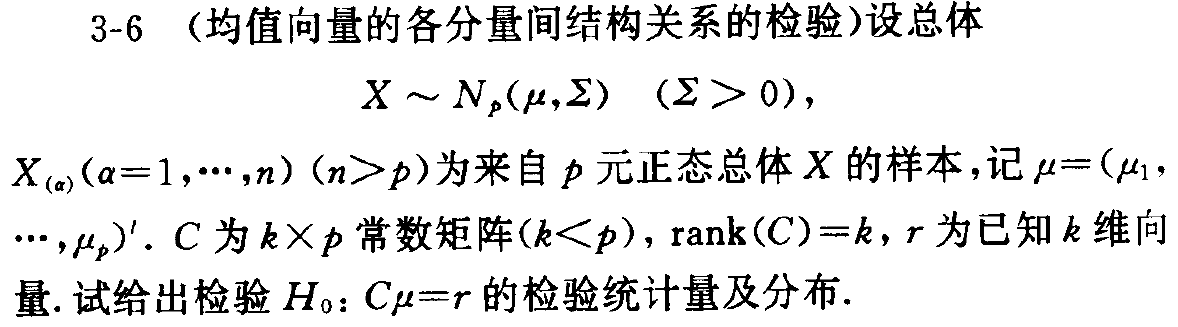
\includegraphics[width=0.7\textwidth]{1.png}
\end{figure}
\begin{solution}
(1) 当$ \Sigma $已知时:

因为$ \mu $的估计量为$ \bar{X} $,故$ C\mu $的估计量为$ C\bar{X} $.由于$$ \bar{X} \sim N_p(\mu,\frac{1}{n}\Sigma)$$可推得$$  C\bar{X} \stackrel{H_0}{\sim} N_k(C\mu=r,\frac{1}{n}C\Sigma C') $$而
$$\sqrt{n}\Sigma ^{-\frac{1}{2}}(\bar{X}-\mu)\sim N_p (0,I_p) $$
故令$$Y=(Y_1,...,Y_k)'=\sqrt{n}(C\Sigma C')^{-\frac{1}{2}}(C\bar{X}-r)\sim N_k (0,I_k) $$
有$$ \sum_{i=1}^{k}Y_i^2=Y'Y=n(C\bar{X}-r)'(C\Sigma C')^{-1}(C\bar{X}-r) \stackrel{H_0}{\sim}\chi^2(k) $$

(2)当$ \Sigma $未知时:
$$ T^2=n(C\bar{X}-r)'(CSC')^{-1}(C\bar{X}-r)\stackrel{H_0}{\sim}T^2(k,n-1) $$
或者
$$F= \frac{n-k}{(n-1)k}T^2=\frac{n(n-k)}{k}(C\bar{X}-r)'(CAC')^{-1}(C\bar{X}-r)\stackrel{H_0}{\sim}F(k,n-k) $$
\end{solution}
\begin{figure}[H]
	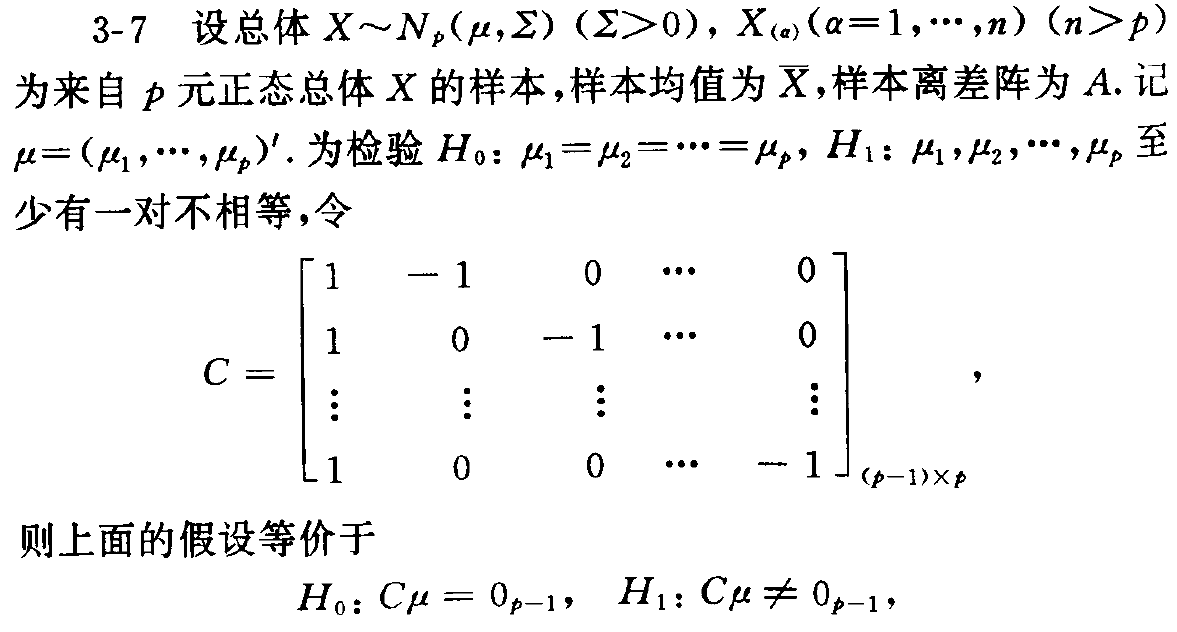
\includegraphics[width=0.7\textwidth]{2.png}
\end{figure}
\begin{figure}[H]
	
\includegraphics[width=0.7\textwidth]{3.png}
\end{figure}
\begin{solution}
似然比统计量
$$ \lambda=
\frac{{\max}_{\theta\in\Theta_0} L(C\mu,C\Sigma C')}{{\max}_{\theta\in\Theta} L(C\mu,C\Sigma C')}
=\frac{L(0,\frac{1}{n}CAC')}{L(C\bar{X},\frac{1}{n}CAC')}\stackrel{H_0}{\sim}\chi^2(\frac{p(p+1)}{2})  $$
\end{solution}

\begin{figure}[H]
	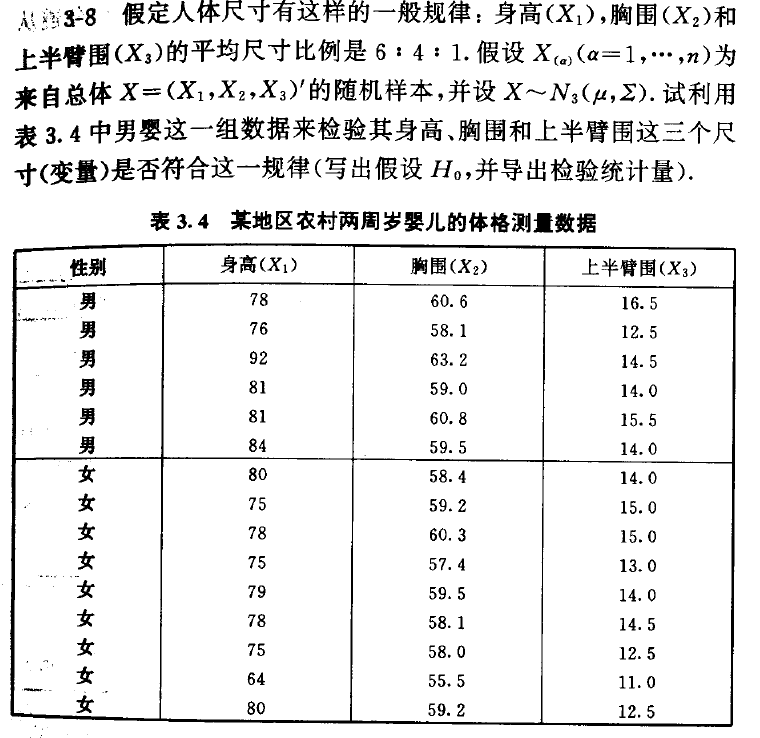
\includegraphics[width=0.7\textwidth]{4.png}
\end{figure}
\begin{solution}
令$ C= \left(
\begin{array}{ccc}
	4 & -6 & 0\\
	1 & 0 & -6\\
\end{array} \right) $,则
$$ H_0: C\mu=\textbf{0} \leftrightarrow H_1:C\mu\neq \textbf{0} $$其中$ \mu=(\mu_1,\mu_2,\mu_3)' $.由于$ \Sigma $未知,故用Hotelling $ T^2 $检验.

$ C\mu $的估计量$ C\bar{X}\sim N_3(C\mu,C\Sigma C') $,$ C\bar{X}\stackrel{H_0}{\sim}N_3(0,C\Sigma C') $.构造检验统计量:
$$T^2=n(C\bar{X}-0)'(CSC')^{-1}(C\bar{X}-0)=n(n-1)(C\bar{X})'(CAC')^{-1}(C\bar{X})\sim T^2(p,n-1) $$

或
$$F=\frac{n-p}{(n-1)p}T^2\stackrel{H_0}{\sim}F(p,n-p)$$其中$ p=3,n=6. $
\end{solution}
\begin{lstlisting}[language=r]
> tige<-read.csv("E:/4.多元统计分析/zuoye/3/1.csv",stringsAsFactors = TRUE)
> print(tige)
   gender X1   X2   X3
1       B 78 60.6 16.5
2       B 76 58.1 12.5
3       B 92 63.2 14.5
......
13      G 75 58.0 12.5
14      G 64 55.5 11.0
15      G 80 59.2 12.5
> X<-data.frame(tige[c(1:6),])
> X<-data.frame(X[,-1])
> a<-colMeans(X)   #样本均值
> a<-as.matrix(a,byrow=TRUE)   
> c<-matrix(data=c(4,-6,0,1,0,-6),byrow=FALSE,ncol=3)    #C矩阵
> A<-5*cov(X)    #样本离差阵
> ca<-c%*%a
> ca2<-t(ca)
> c2<-t(c)   #C的转置
> CAC<-c%*%A%*%c2
> CAC3<-solve(CAC)
> F<-6*ca2%*%CAC3%*%ca    #F检验统计量
> F
         [,1]
[1,] 290.0087
> 1-pf(F,3,3)   #p值
             [,1]
[1,] 0.0003416187   #小于0.0005,故否定原假设,认为三个尺寸不符合这一规律.
\end{lstlisting}


\begin{figure}[H]
	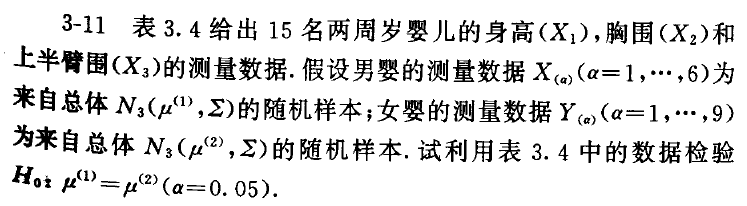
\includegraphics[width=0.7\textwidth]{5.png}
\end{figure}
\begin{solution}
$ n_1=6, n_2=9$,同方差的两正态总体均值向量检验的检验统计量为
$$\frac{n_1n_2}{n_1+n_2}(\bar{X}-\bar{Y})'(\frac{A_1+A_2}{n_1+n_2-2})^{-1}(\bar{X}-\bar{Y})\stackrel{H_0}{\sim}T^2(p,n_1+n_2-2) $$
\end{solution}
\begin{lstlisting}[language=r]
> Y<-data.frame(tige[c(7:15),-1])
> a1<-colMeans(X)  
> a2<-colMeans(Y)
> a1<-as.matrix(a1,byrow=TRUE)  #X的均值向量
> a2<-as.matrix(a2,byrow=TRUE)  #Y的均值向量
> A1<-5*cov(X)   #X的样本离差阵
> A2<-8*cov(Y)   #Y的样本离差阵
> a1.a2<-a1-a2
> a1.a2_t<-t(a1.a2)
> A1.A2<-solve((A1+A2)/13)  #混合样本协方差阵的逆
> T2<-(6*9/15)*a1.a2_t%*%A1.A2%*%a1.a2
> T2
         [,1]
[1,] 5.311726
> F<-11/13/3*T2    #转换为F分布
> F
         [,1]
[1,] 1.498179
> 1-pf(F,3,11)
          [,1]
[1,] 0.2692616    #p值大于0.05,故接受H_0
\end{lstlisting}
\newpage
\begin{figure}[H]
	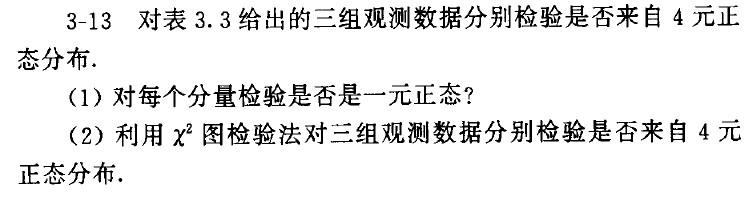
\includegraphics[width=0.7\textwidth]{6.png}
\end{figure}
\begin{tcolorbox}[colback=black!4!white,colframe=black!40]
\begin{figure}[H]
	\centering
	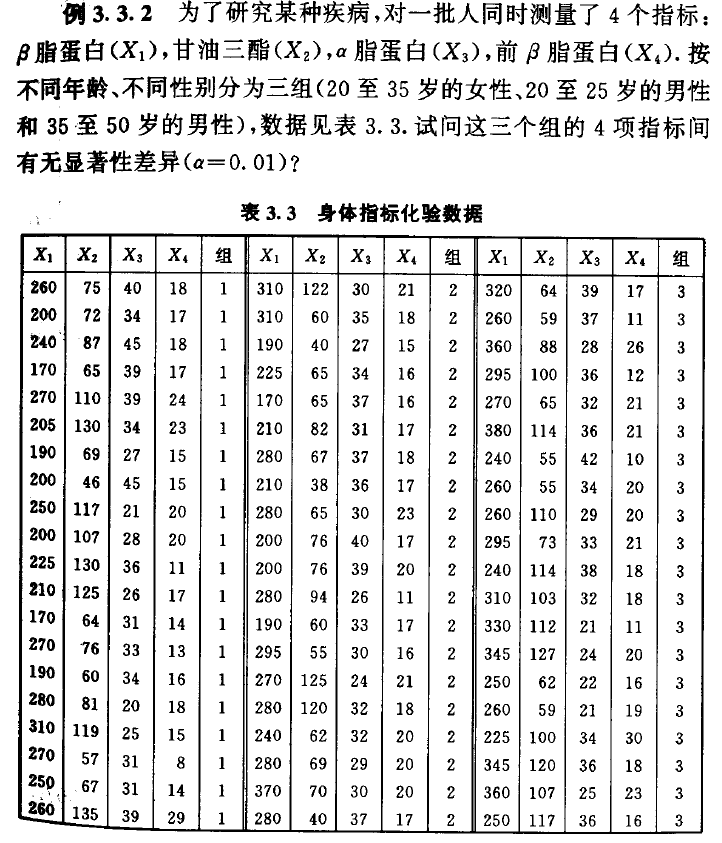
\includegraphics[width=0.7\textwidth]{7.png}
\end{figure}
\end{tcolorbox}

\begin{solution}

\subsection*{(第一问):}
\subsubsection*{1.1直方图}
\end{solution}
\begin{figure}[H]
	\centering
	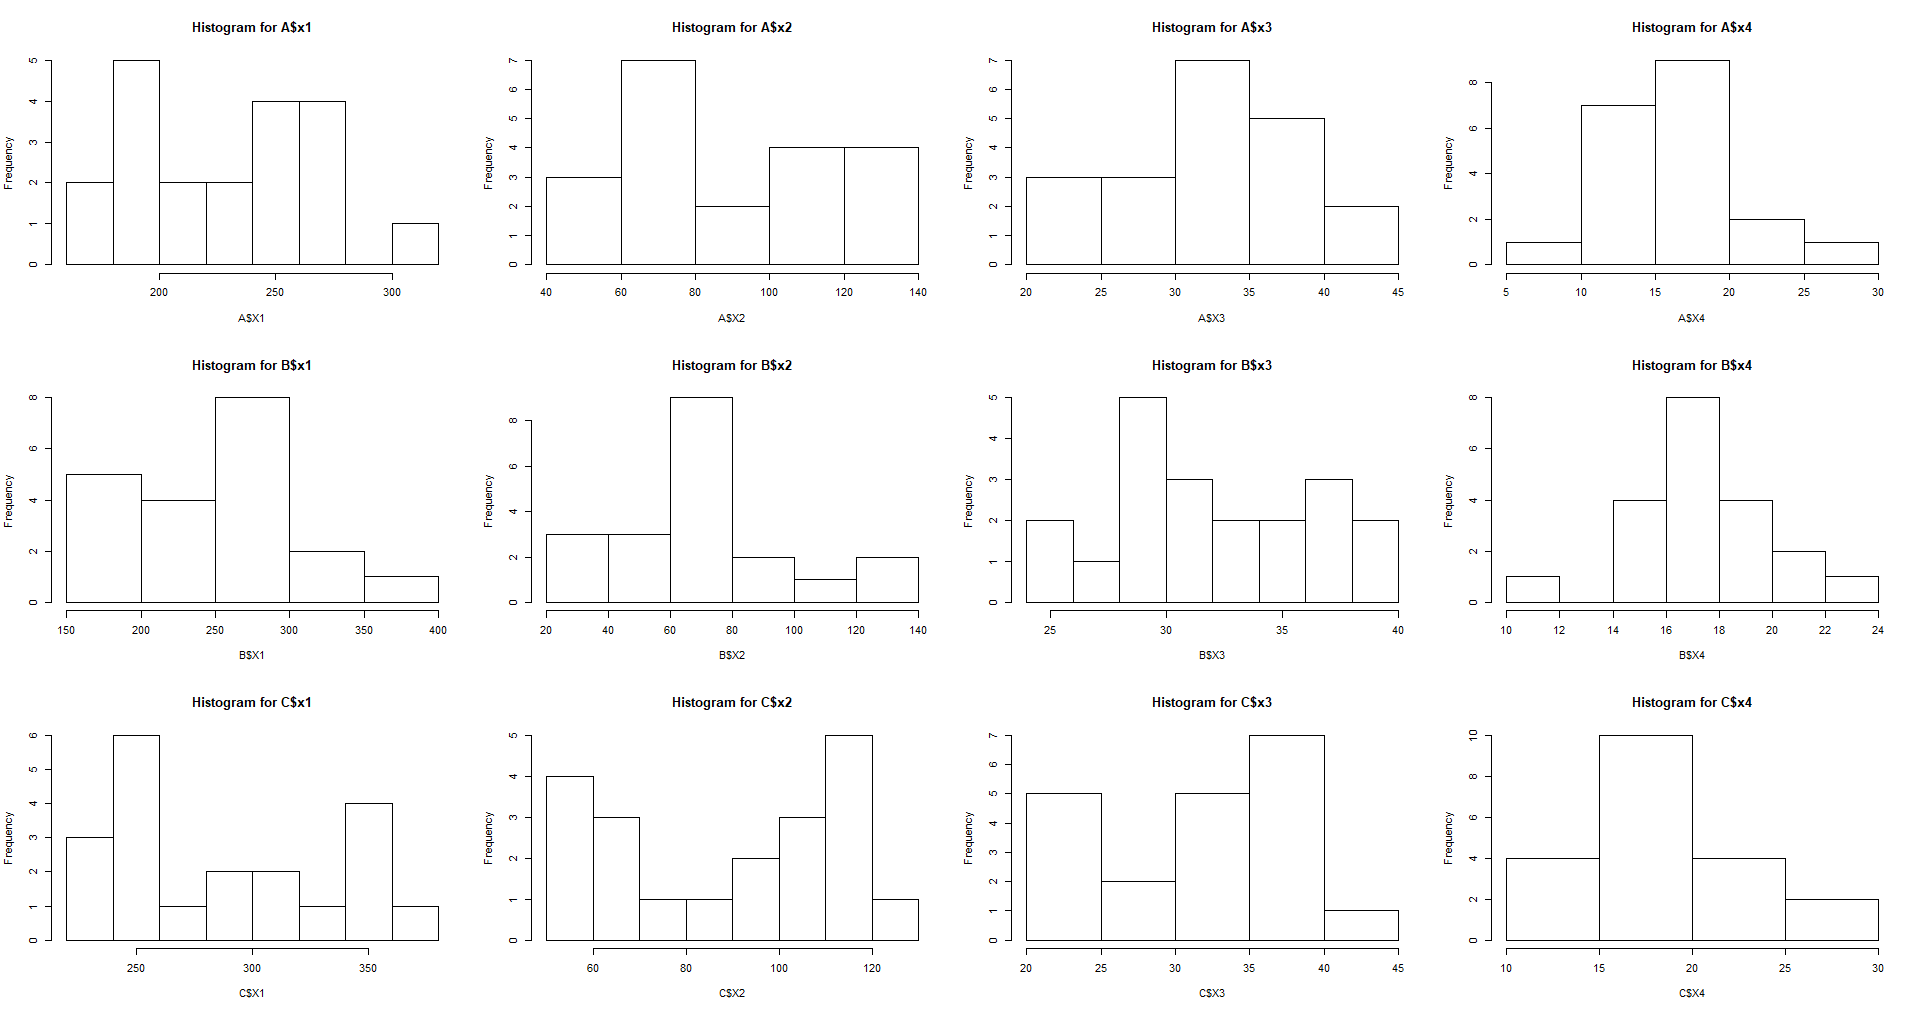
\includegraphics[width=\textwidth]{8.png}
\end{figure}
由图观察,组1的第4特征和组2的第4特征接近一元正态.

\subsubsection*{1.2 QQ图}

\begin{figure}[H]
	\centering
	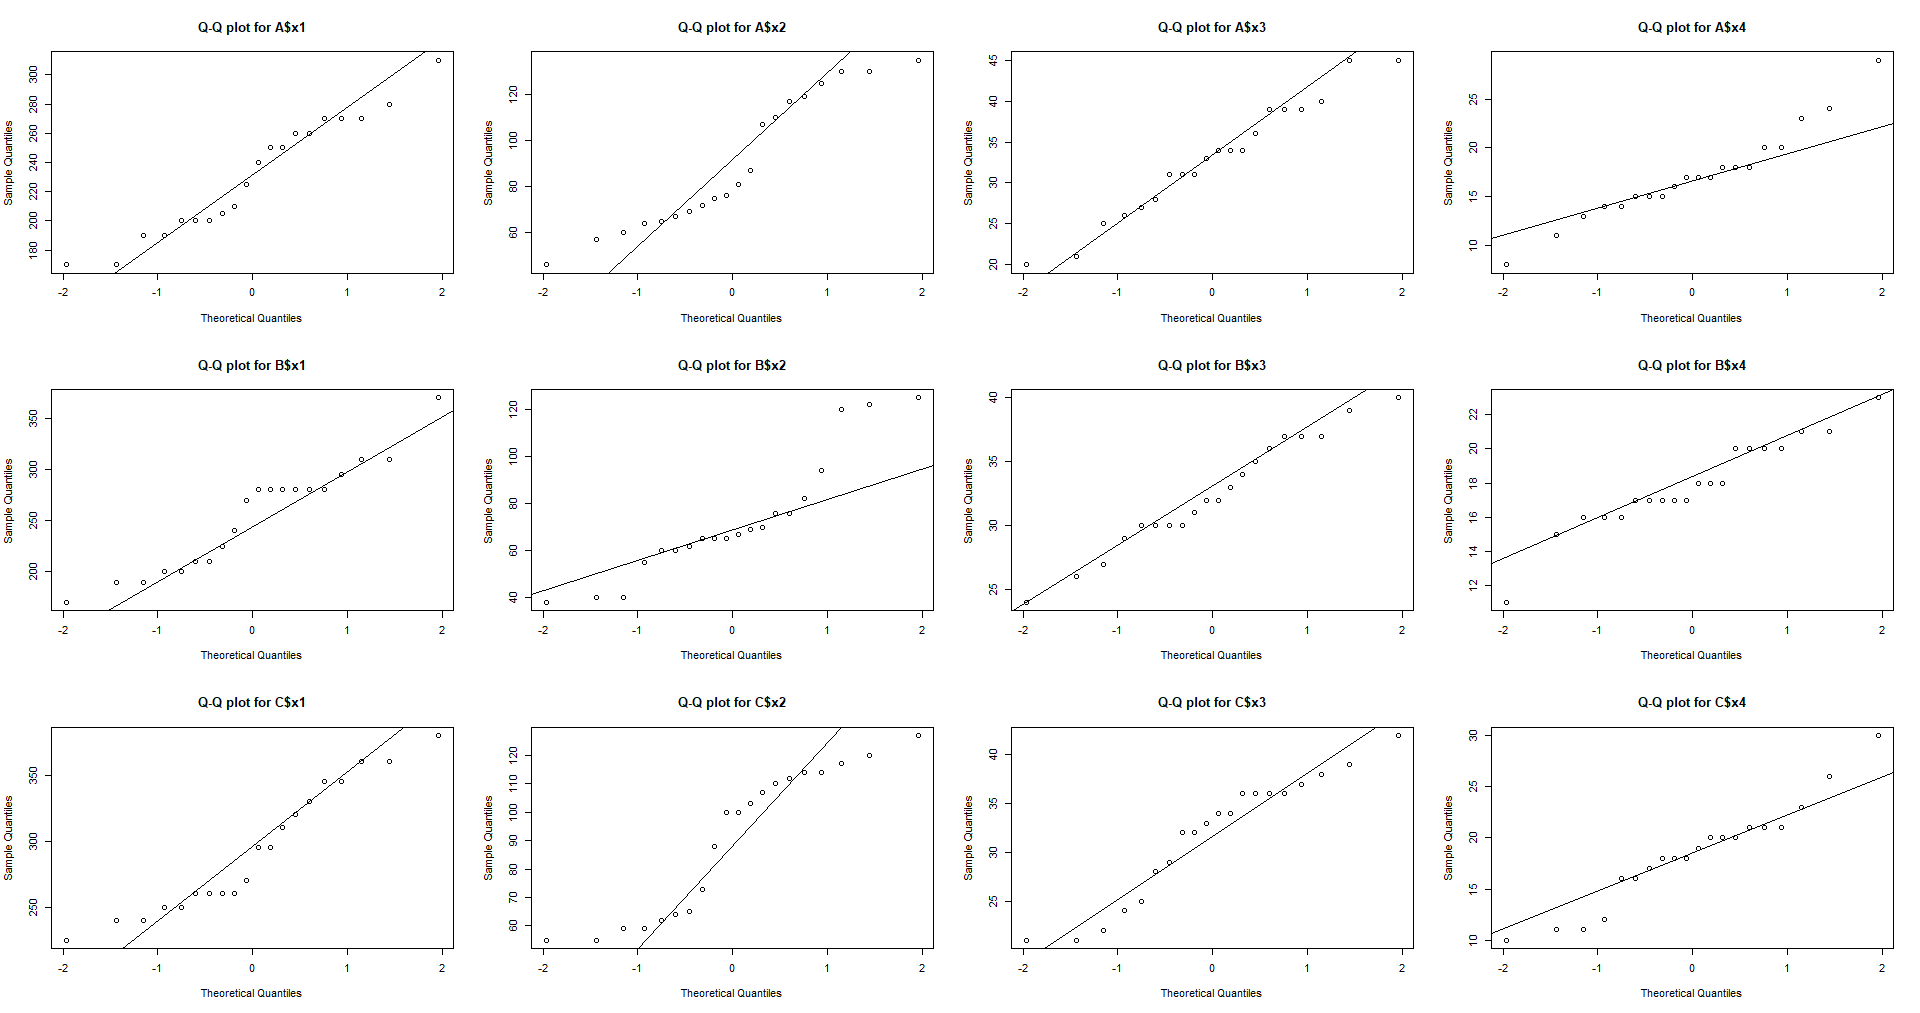
\includegraphics[width=\textwidth]{9.png}
\end{figure}
由图观察,组1的第3特征和组2的第4特征接近一元正态.

\subsubsection*{1.3 偏度和峰度}

由结果(结果见附录),组1的第4特征,组2的第4特征,组3的第4特征接近一元正态.

\subsubsection*{1.4 统计检验}
\textbf{(1)Shapiro-Wilks test}


由检验结果(见附录),组1的第3特征,组1的第4特征,组2的第3特征,组3的第4特征接近一元正态.

\textbf{(2)Kolmogorov-Smirnov test}


由检验结果(见附录),组1的第3特征,组2的第4特征接近一元正态.

\textbf{(3)Cramer-von Mises test}

由检验结果(见附录),组1的第3特征,组2的第3特征接近一元正态.

\textbf{(4)Anderson-Darling test}

由检验结果(见附录),组1的第3特征,组2的第3特征接近一元正态.


\subsection*{(第二问):}

1.第一组

\begin{lstlisting}[language=r]
> y <- A
> cm <- colMeans(y)
> S <- cov(y)
> d <- apply(y, 1, function(y) t(y - cm) %*% solve(S) %*% (y - cm))
> plot(qc <- qchisq((1:nrow(y) - 1/2) / nrow(y), df = 4), sd <- sort(d),
+      xlab = expression(paste(chi[4]^2, " Quantile")),
+      ylab = "Ordered distances", xlim = range(qc) * c(1, 1.1))
> abline(a = 0, b = 1)
\end{lstlisting}
\begin{figure}[H]
	\centering
	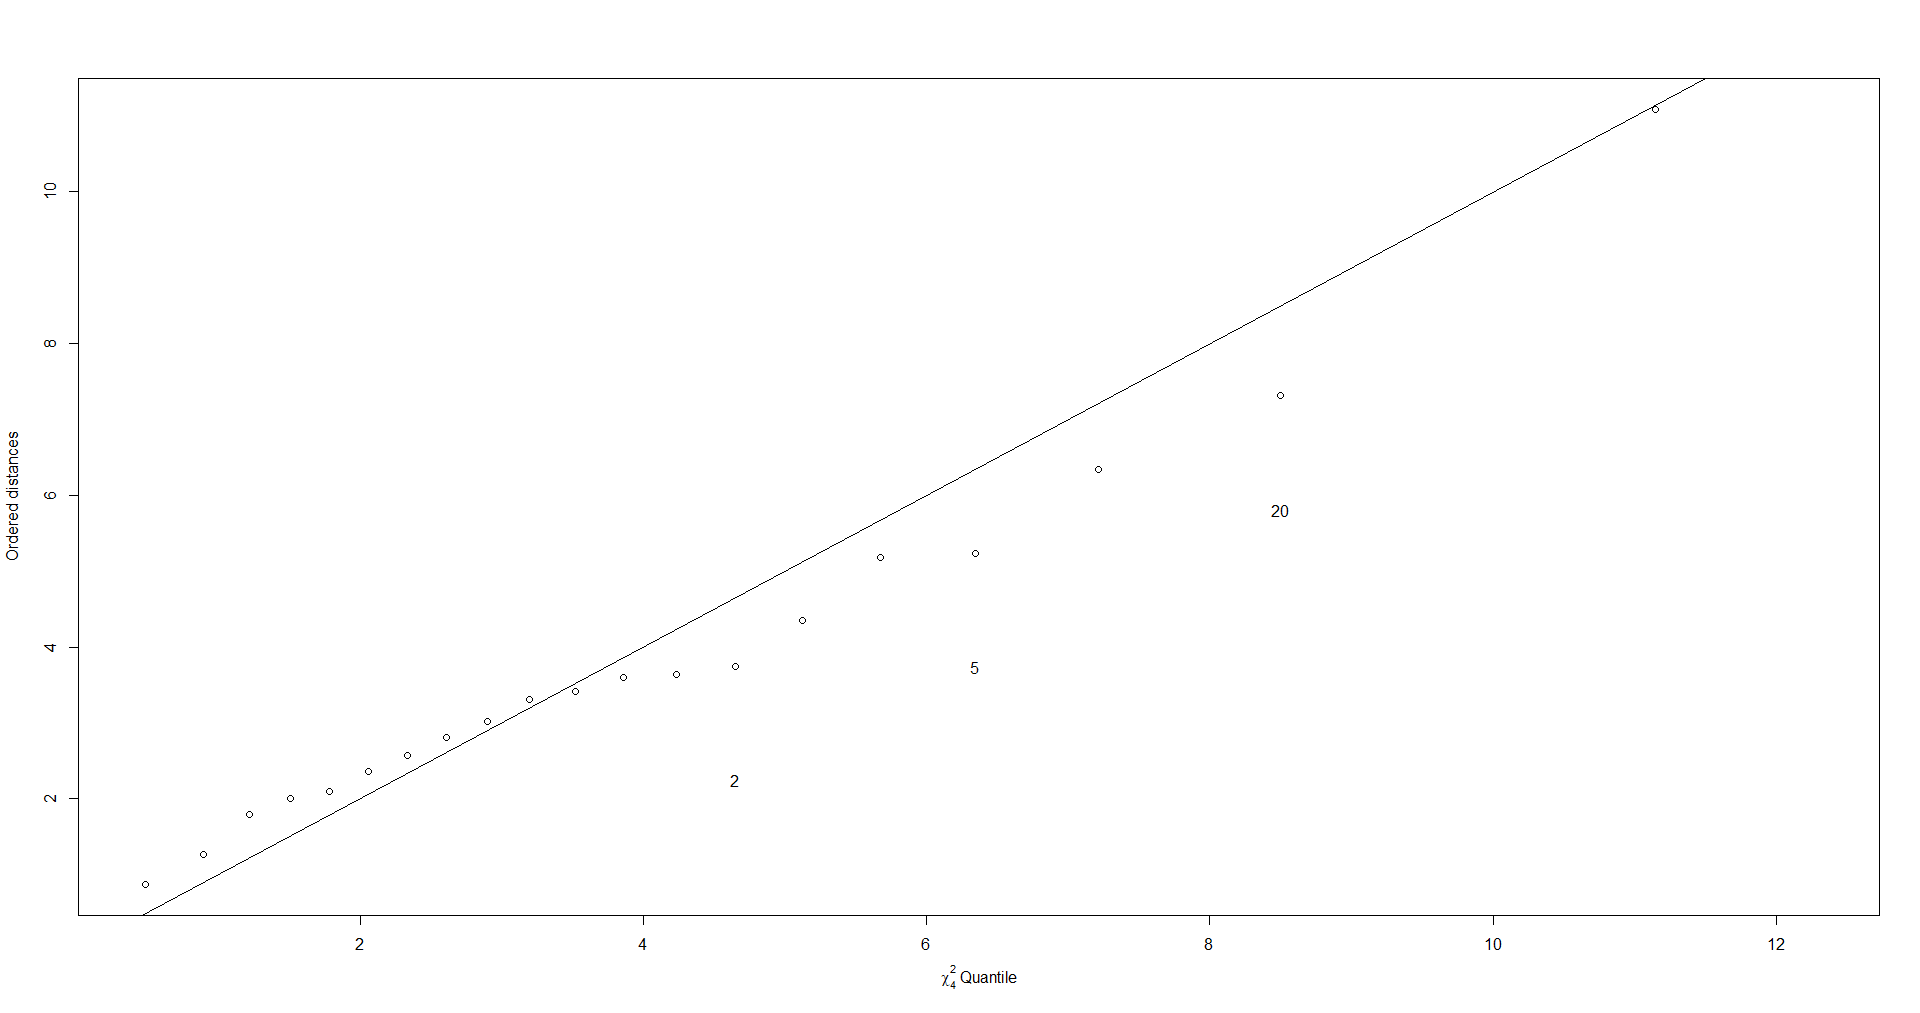
\includegraphics[width=\textwidth]{10.png}
\end{figure}
拒绝正态性假设.\\

2.第二组

\begin{lstlisting}[language=r]
> y <- B
> cm <- colMeans(y)
> S <- cov(y)
> d <- apply(y, 1, function(y) t(y - cm) %*% solve(S) %*% (y - cm))
> plot(qc <- qchisq((1:nrow(y) - 1/2) / nrow(y), df = 4), sd <- sort(d),
+      xlab = expression(paste(chi[4]^2, " Quantile")),
+      ylab = "Ordered distances", xlim = range(qc) * c(1, 1.1))
> abline(a = 0, b = 1)
\end{lstlisting}
\begin{figure}[H]
	\centering
	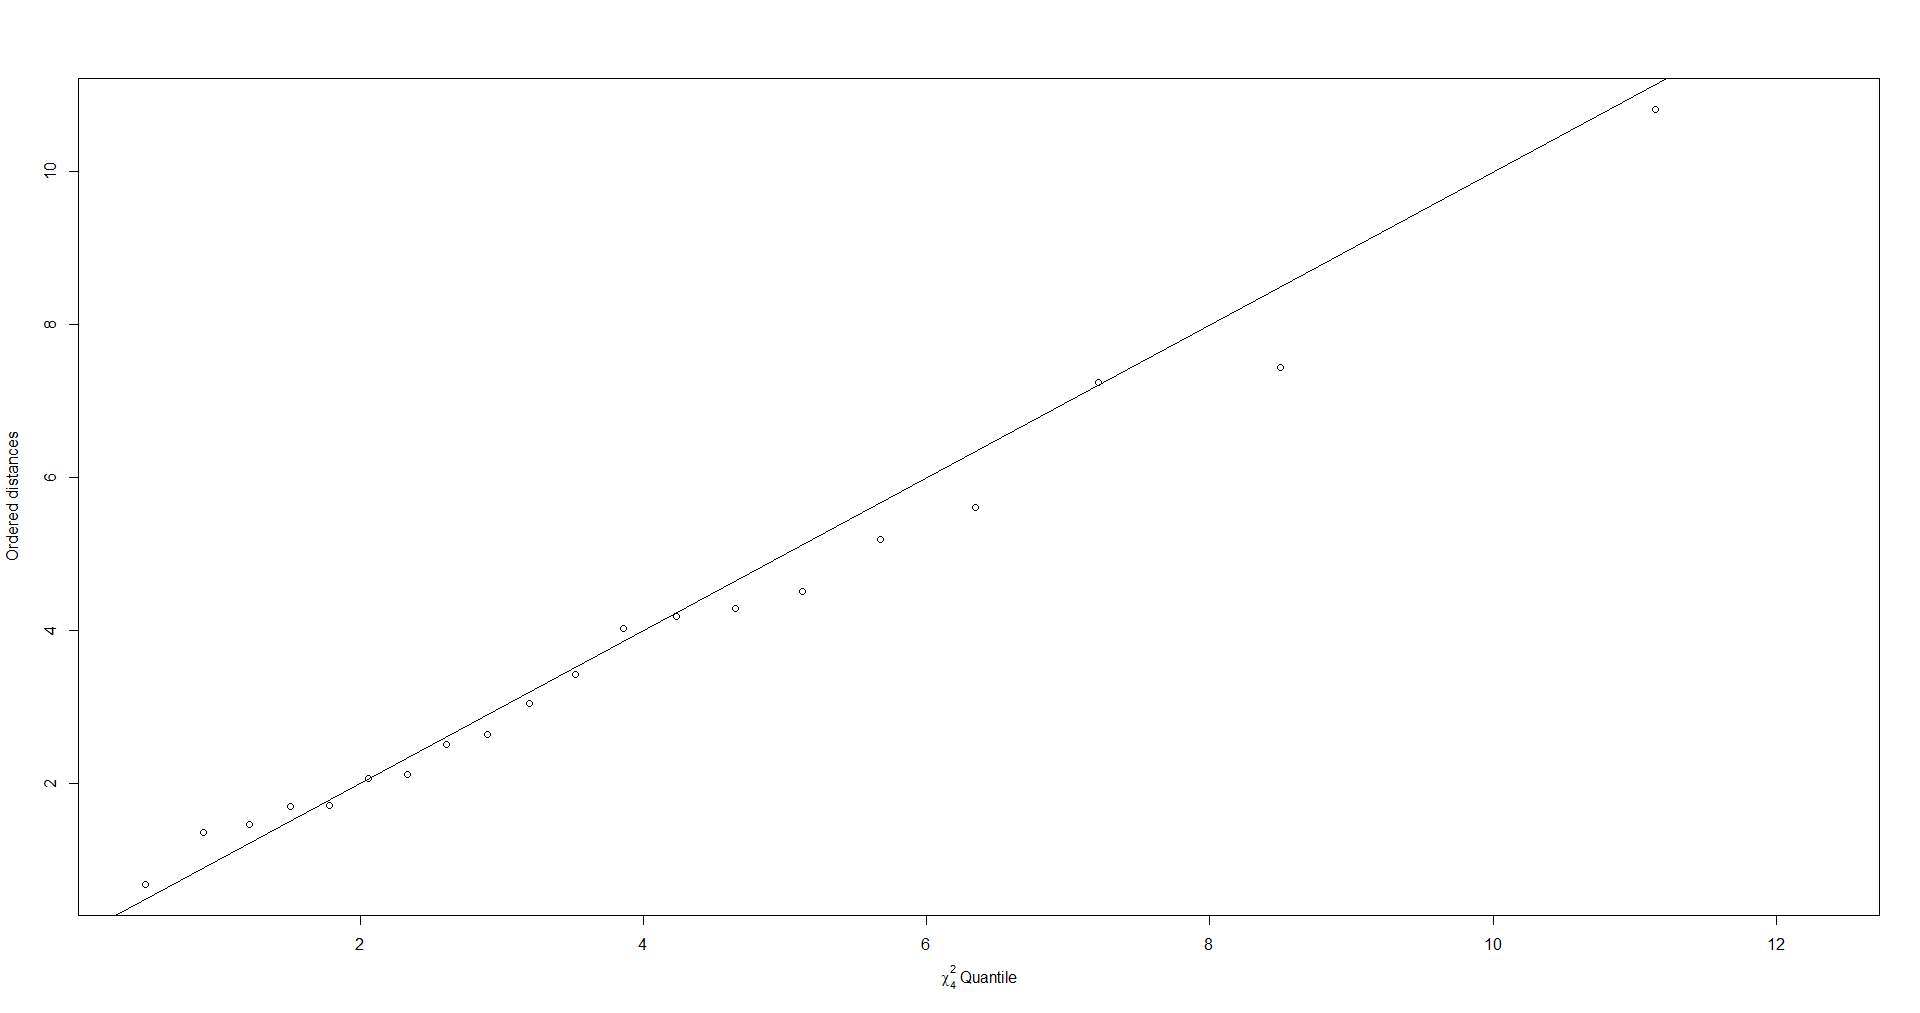
\includegraphics[width=\textwidth]{11.png}
\end{figure}
勉强接受正态性假设.\\

3.第三组

\begin{lstlisting}[language=r]
> y <- C
> cm <- colMeans(y)
> S <- cov(y)
> d <- apply(y, 1, function(y) t(y - cm) %*% solve(S) %*% (y - cm))
> plot(qc <- qchisq((1:nrow(y) - 1/2) / nrow(y), df = 4), sd <- sort(d),
+      xlab = expression(paste(chi[4]^2, " Quantile")),
+      ylab = "Ordered distances", xlim = range(qc) * c(1, 1.1))
> abline(a = 0, b = 1)
\end{lstlisting}
\begin{figure}[H]
	\centering
	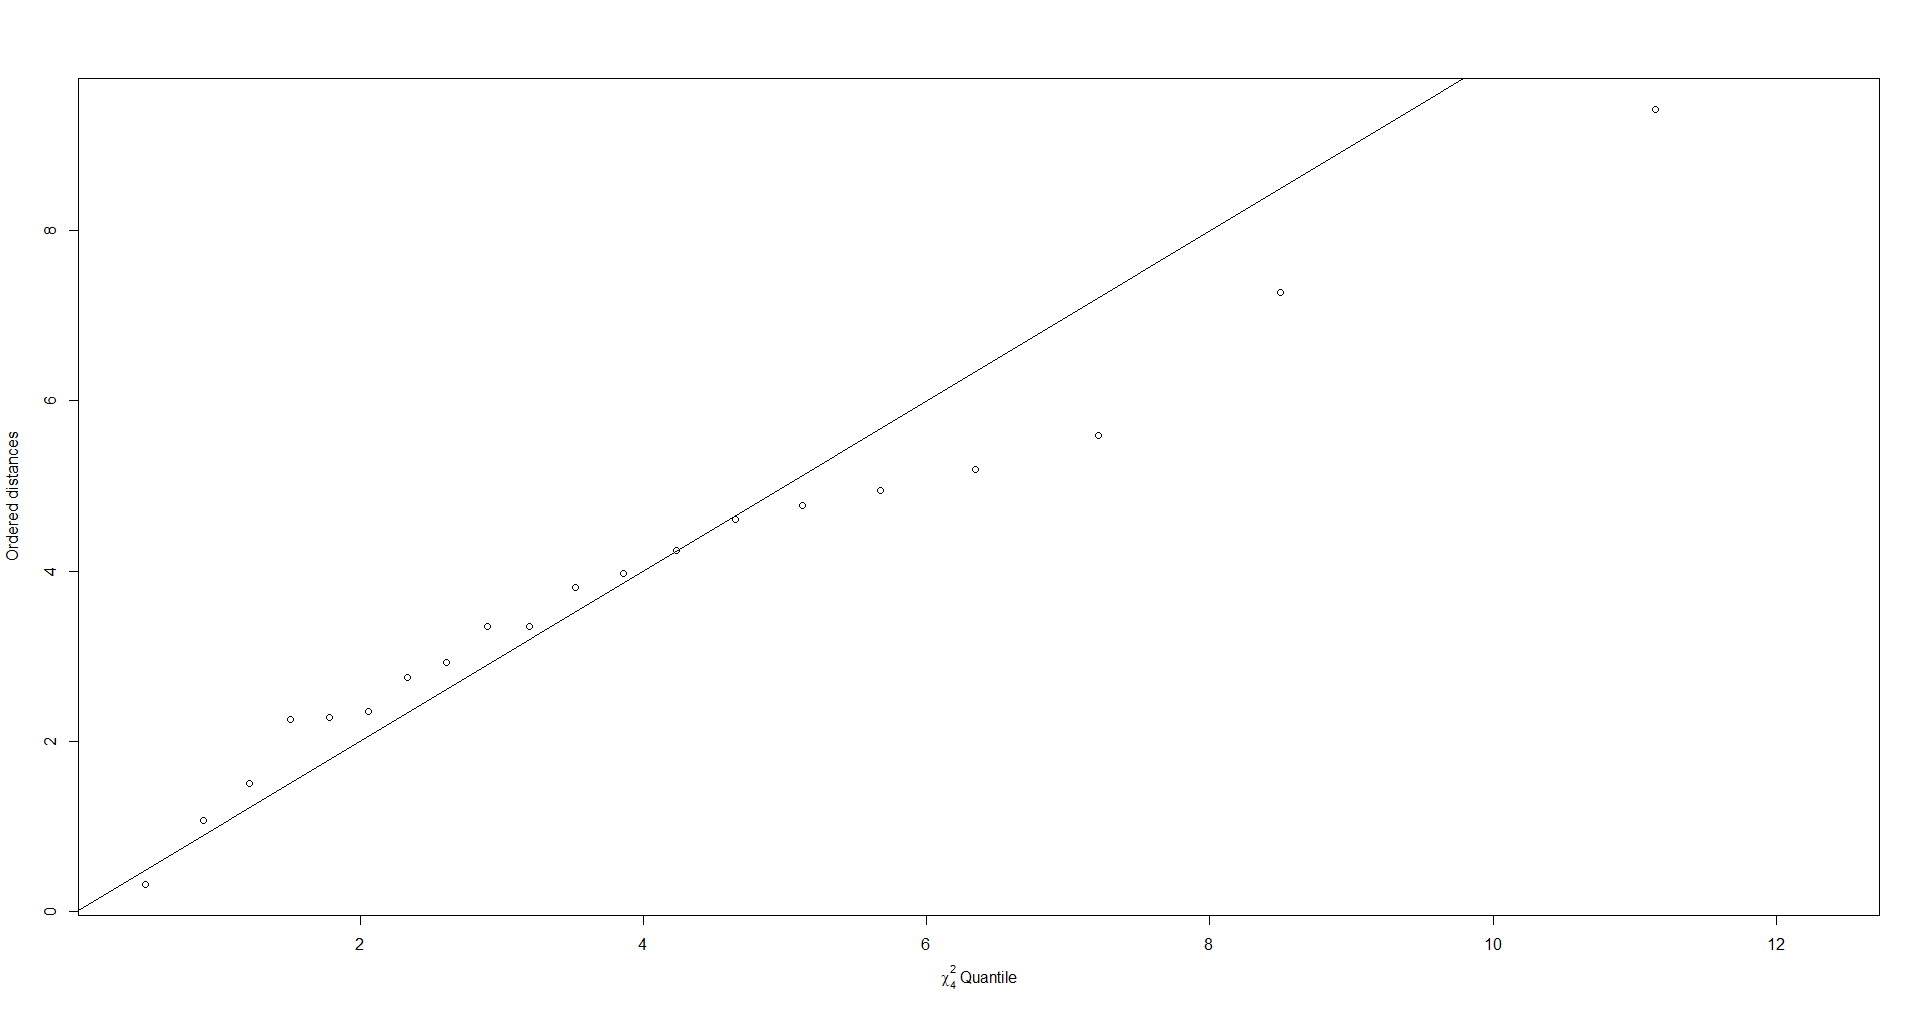
\includegraphics[width=\textwidth]{12.png}
\end{figure}
拒绝正态性假设.

\newpage
\centering\textbf{\Large 附录}


\begin{appendices}
\section{3-13 1.1 直方图}
\begin{lstlisting}[language=r]
> data<-read.csv("E:/4.多元统计分析/zuoye/3/2.csv",stringsAsFactors = TRUE)
> A<-data.frame(data[c(1:20),-1])     #将三个组分出来
> B<-data.frame(data[c(21:40),-1])
> C<-data.frame(data[c(41:60),-1])
> par(mfrow=c(3,4))
> hist(A$X1,main="Histogram for A$x1")
> hist(A$X2,main="Histogram for A$x2")
> hist(A$X3,main="Histogram for A$x3")
> hist(A$X4,main="Histogram for A$x4")
> hist(B$X1,main="Histogram for B$x1")
> hist(B$X2,main="Histogram for B$x2")
> hist(B$X3,main="Histogram for B$x3")
> hist(B$X4,main="Histogram for B$x4")
> hist(C$X1,main="Histogram for C$x1")
> hist(C$X2,main="Histogram for C$x2")
> hist(C$X3,main="Histogram for C$x3")
> hist(C$X4,main="Histogram for C$x4")
\end{lstlisting}
\section{3-13 1.2 QQ图}
\begin{lstlisting}[language=r]
par(mfrow=c(3,4))
qqnorm(A$X1,main="Q-Q plot for A$x1"); qqline(A$X1)
qqnorm(A$X2,main="Q-Q plot for A$x2"); qqline(A$X2)
qqnorm(A$X3,main="Q-Q plot for A$x3"); qqline(A$X3)
qqnorm(A$X4,main="Q-Q plot for A$x4"); qqline(A$X4)
qqnorm(B$X1,main="Q-Q plot for B$x1"); qqline(B$X1)
qqnorm(B$X2,main="Q-Q plot for B$x2"); qqline(B$X2)
qqnorm(B$X3,main="Q-Q plot for B$x3"); qqline(B$X3)
qqnorm(B$X4,main="Q-Q plot for B$x4"); qqline(B$X4)
qqnorm(C$X1,main="Q-Q plot for C$x1"); qqline(C$X1)
qqnorm(C$X2,main="Q-Q plot for C$x2"); qqline(C$X2)
qqnorm(C$X3,main="Q-Q plot for C$x3"); qqline(C$X3)
qqnorm(C$X4,main="Q-Q plot for C$x4"); qqline(C$X4)
\end{lstlisting}
\section{3-13 1.3 偏度和峰度}
\begin{lstlisting}[language=r]
> library(moments)
> skewness(A$X1); kurtosis(A$X1)
[1] 0.1204204
[1] 1.933383
> skewness(A$X2); kurtosis(A$X2)
[1] 0.2773125
[1] 1.587005
> skewness(A$X3); kurtosis(A$X3)
[1] -0.05769829
[1] 2.307432
> skewness(A$X4); kurtosis(A$X4)
[1] 0.601332
[1] 3.789564
> skewness(B$X1); kurtosis(B$X1)
[1] 0.2049252
[1] 2.363692
> skewness(B$X2); kurtosis(B$X2)
[1] 0.8553859
[1] 3.002884
> skewness(B$X3); kurtosis(B$X3)
[1] -0.04971583
[1] 2.19002
> skewness(B$X4); kurtosis(B$X4)
[1] -0.4271917
[1] 3.707689
> skewness(C$X1); kurtosis(C$X1)
[1] 0.3598219
[1] 1.764333
> skewness(C$X2); kurtosis(C$X2)
[1] -0.1937781
[1] 1.401273
> skewness(C$X3); kurtosis(C$X3)
[1] -0.4423124
[1] 2.038037
> skewness(C$X4); kurtosis(C$X4)
[1] 0.2004094
[1] 3.058989
\end{lstlisting}
\section{3-13 1.4.1 Shapiro-Wilks test}
\begin{lstlisting}[language=r]
> shapiro.test(A$X1)

Shapiro-Wilk normality test

data:  A$X1
W = 0.94438, p-value = 0.2898

> shapiro.test(A$X2)

Shapiro-Wilk normality test

data:  A$X2
W = 0.90348, p-value = 0.04795

> shapiro.test(A$X3)

Shapiro-Wilk normality test

data:  A$X3
W = 0.97035, p-value = 0.7622

> shapiro.test(A$X4)

Shapiro-Wilk normality test

data:  A$X4
W = 0.9573, p-value = 0.4914

> shapiro.test(B$X1)

Shapiro-Wilk normality test

data:  B$X1
W = 0.93141, p-value = 0.1644

> shapiro.test(B$X2)

Shapiro-Wilk normality test

data:  B$X2
W = 0.87954, p-value = 0.01736

> shapiro.test(B$X3)

Shapiro-Wilk normality test

data:  B$X3
W = 0.97246, p-value = 0.8057

> shapiro.test(B$X4)

Shapiro-Wilk normality test

data:  B$X4
W = 0.94251, p-value = 0.2674

> shapiro.test(C$X1)

Shapiro-Wilk normality test

data:  C$X1
W = 0.92007, p-value = 0.09939

> shapiro.test(C$X2)

Shapiro-Wilk normality test

data:  C$X2
W = 0.87082, p-value = 0.01215

> shapiro.test(C$X3)

Shapiro-Wilk normality test

data:  C$X3
W = 0.92527, p-value = 0.1252

> shapiro.test(C$X4)

Shapiro-Wilk normality test

data:  C$X4
W = 0.9509, p-value = 0.381

\end{lstlisting}
\section{3-13 1.4.2 One-sample Kolmogorov-Smirnov test}
\begin{lstlisting}[language=r]
> library(nortest)  # package for normality tests
> ks.test(A$X1,"pnorm",mean(A$X1),sqrt(var(A$X1)))

One-sample Kolmogorov-Smirnov test

data:  A$X1
D = 0.14982, p-value = 0.7604
alternative hypothesis: two-sided

Warning message:
In ks.test(A$X1, "pnorm", mean(A$X1), sqrt(var(A$X1))) :
Kolmogorov - Smirnov检验里不应该有连结
> ks.test(A$X2,"pnorm",mean(A$X2),sqrt(var(A$X2)))

One-sample Kolmogorov-Smirnov test

data:  A$X2
D = 0.18174, p-value = 0.5235
alternative hypothesis: two-sided

Warning message:
In ks.test(A$X2, "pnorm", mean(A$X2), sqrt(var(A$X2))) :
Kolmogorov - Smirnov检验里不应该有连结
> ks.test(A$X3,"pnorm",mean(A$X3),sqrt(var(A$X3)))

One-sample Kolmogorov-Smirnov test

data:  A$X3
D = 0.10512, p-value = 0.9799
alternative hypothesis: two-sided

Warning message:
In ks.test(A$X3, "pnorm", mean(A$X3), sqrt(var(A$X3))) :
Kolmogorov - Smirnov检验里不应该有连结
> ks.test(A$X4,"pnorm",mean(A$X4),sqrt(var(A$X4)))

One-sample Kolmogorov-Smirnov test

data:  A$X4
D = 0.17354, p-value = 0.5835
alternative hypothesis: two-sided

Warning message:
In ks.test(A$X4, "pnorm", mean(A$X4), sqrt(var(A$X4))) :
Kolmogorov - Smirnov检验里不应该有连结
> ks.test(B$X1,"pnorm",mean(B$X1),sqrt(var(B$X1)))

One-sample Kolmogorov-Smirnov test

data:  B$X1
D = 0.19427, p-value = 0.4372
alternative hypothesis: two-sided

Warning message:
In ks.test(B$X1, "pnorm", mean(B$X1), sqrt(var(B$X1))) :
Kolmogorov - Smirnov检验里不应该有连结
> ks.test(B$X2,"pnorm",mean(B$X2),sqrt(var(B$X2)))

One-sample Kolmogorov-Smirnov test

data:  B$X2
D = 0.19605, p-value = 0.4256
alternative hypothesis: two-sided

Warning message:
In ks.test(B$X2, "pnorm", mean(B$X2), sqrt(var(B$X2))) :
Kolmogorov - Smirnov检验里不应该有连结
> ks.test(B$X3,"pnorm",mean(B$X3),sqrt(var(B$X3)))

One-sample Kolmogorov-Smirnov test

data:  B$X3
D = 0.11193, p-value = 0.9636
alternative hypothesis: two-sided

Warning message:
In ks.test(B$X3, "pnorm", mean(B$X3), sqrt(var(B$X3))) :
Kolmogorov - Smirnov检验里不应该有连结
> ks.test(B$X4,"pnorm",mean(B$X4),sqrt(var(B$X4)))

One-sample Kolmogorov-Smirnov test

data:  B$X4
D = 0.137, p-value = 0.8471
alternative hypothesis: two-sided

Warning message:
In ks.test(B$X4, "pnorm", mean(B$X4), sqrt(var(B$X4))) :
Kolmogorov - Smirnov检验里不应该有连结
> ks.test(C$X1,"pnorm",mean(C$X1),sqrt(var(C$X1)))

One-sample Kolmogorov-Smirnov test

data:  C$X1
D = 0.20397, p-value = 0.3761
alternative hypothesis: two-sided

Warning message:
In ks.test(C$X1, "pnorm", mean(C$X1), sqrt(var(C$X1))) :
Kolmogorov - Smirnov检验里不应该有连结
> ks.test(C$X2,"pnorm",mean(C$X2),sqrt(var(C$X2)))

One-sample Kolmogorov-Smirnov test

data:  C$X2
D = 0.19913, p-value = 0.4059
alternative hypothesis: two-sided

Warning message:
In ks.test(C$X2, "pnorm", mean(C$X2), sqrt(var(C$X2))) :
Kolmogorov - Smirnov检验里不应该有连结
> ks.test(C$X3,"pnorm",mean(C$X3),sqrt(var(C$X3)))

One-sample Kolmogorov-Smirnov test

data:  C$X3
D = 0.16575, p-value = 0.6419
alternative hypothesis: two-sided

Warning message:
In ks.test(C$X3, "pnorm", mean(C$X3), sqrt(var(C$X3))) :
Kolmogorov - Smirnov检验里不应该有连结
> ks.test(C$X4,"pnorm",mean(C$X4),sqrt(var(C$X4)))

One-sample Kolmogorov-Smirnov test

data:  C$X4
D = 0.15187, p-value = 0.7455
alternative hypothesis: two-sided

Warning message:
In ks.test(C$X4, "pnorm", mean(C$X4), sqrt(var(C$X4))) :
Kolmogorov - Smirnov检验里不应该有连结
\end{lstlisting}
\section{3-13 1.4.3 Cramer-von Mises normality test}
\begin{lstlisting}[language=r]
> cvm.test(A$X1)

Cramer-von Mises normality test

data:  A$X1
W = 0.086853, p-value = 0.1584

> cvm.test(A$X2)

Cramer-von Mises normality test

data:  A$X2
W = 0.14504, p-value = 0.02482

> cvm.test(A$X3)

Cramer-von Mises normality test

data:  A$X3
W = 0.029414, p-value = 0.8454

> cvm.test(A$X4)

Cramer-von Mises normality test

data:  A$X4
W = 0.074724, p-value = 0.2295

> cvm.test(B$X1)

Cramer-von Mises normality test

data:  B$X1
W = 0.12397, p-value = 0.04817

> cvm.test(B$X2)

Cramer-von Mises normality test

data:  B$X2
W = 0.16261, p-value = 0.01441

> cvm.test(B$X3)

Cramer-von Mises normality test

data:  B$X3
W = 0.041269, p-value = 0.6392

> cvm.test(B$X4)

Cramer-von Mises normality test

data:  B$X4
W = 0.085822, p-value = 0.1635

> cvm.test(C$X1)

Cramer-von Mises normality test

data:  C$X1
W = 0.11306, p-value = 0.06823

> cvm.test(C$X2)

Cramer-von Mises normality test

data:  C$X2
W = 0.17689, p-value = 0.00932

> cvm.test(C$X3)

Cramer-von Mises normality test

data:  C$X3
W = 0.10375, p-value = 0.09207

> cvm.test(C$X4)

Cramer-von Mises normality test

data:  C$X4
W = 0.0695, p-value = 0.2695
\end{lstlisting}
\section{3-13 1.4.4 Anderson-Darling normality test}
\begin{lstlisting}[language=r]
> ad.test(A$X1)

Anderson-Darling normality test

data:  A$X1
A = 0.48879, p-value = 0.1974

> ad.test(A$X2)

Anderson-Darling normality test

data:  A$X2
A = 0.80834, p-value = 0.02999

> ad.test(A$X3)

Anderson-Darling normality test

data:  A$X3
A = 0.20767, p-value = 0.8443

> ad.test(A$X4)

Anderson-Darling normality test

data:  A$X4
A = 0.42246, p-value = 0.2906

> ad.test(B$X1)

Anderson-Darling normality test

data:  B$X1
A = 0.67108, p-value = 0.06764

> ad.test(B$X2)

Anderson-Darling normality test

data:  B$X2
A = 0.97028, p-value = 0.0115

> ad.test(B$X3)

Anderson-Darling normality test

data:  B$X3
A = 0.2485, p-value = 0.7141

> ad.test(B$X4)

Anderson-Darling normality test

data:  B$X4
A = 0.52176, p-value = 0.162

> ad.test(C$X1)

Anderson-Darling normality test

data:  C$X1
A = 0.65859, p-value = 0.07283

> ad.test(C$X2)

Anderson-Darling normality test

data:  C$X2
A = 1.0481, p-value = 0.007258

> ad.test(C$X3)

Anderson-Darling normality test

data:  C$X3
A = 0.61015, p-value = 0.09707

> ad.test(C$X4)

Anderson-Darling normality test

data:  C$X4
A = 0.43689, p-value = 0.2674
\end{lstlisting}

\end{appendices}
\end{document}